\documentclass{article}

\usepackage[margin=1in]{geometry}
\usepackage{wrapfig}
\usepackage{tkz-euclide}
\usepackage{csquotes}
\usepackage{hyperref}
\usepackage{graphicx}
\usepackage{siunitx}

\title{2021 Castro Valley Junior Math Tournament Problems}
\author{}
\date{}

\begin{document}
\maketitle

\section*{Mooving Cow}
Bessie the Cow is $5$ meters north of Farmer Pearson's house.
She starts running east at $2$ meters per second.
After how many seconds will she be exactly $10$ meters away from Farmer John's house?
Express your answer in exact form.

\section*{Cowangle}
\begin{wrapfigure}{r}{0.35\linewidth}
	\vspace{-20pt}
	\centering
	\begin{tikzpicture}
		\tkzDefPoint(110:2){A}
		\tkzDefPoint(180:2){B}
		\tkzDefPoint(0:2){C}

		\tkzDefPointBy[projection=onto B--C](A)
		\tkzGetPoint{X}

		\tkzDrawPolygon(A,B,C)
		\tkzDrawSegment(A,X)
		\tkzLabelPoints[above](A)
		\tkzLabelPoints[left](B)
		\tkzLabelPoints[right](C)
		\tkzLabelPoints[below](X)
		\tkzMarkRightAngle(B,A,C)
		\tkzMarkRightAngle(A,X,C)
		\tkzLabelLine[above left](A,B){$7$}
		\tkzLabelLine[above right](A,C){$10$}
		\tkzLabelLine[right](A,X){?}
	\end{tikzpicture}
	\vspace{-20pt}
\end{wrapfigure}
Bessie the Cow found the following right triangle $ABC$.
The distance from point $A$ to point $B$ is $7$, and the distance from point $A$ to point $C$ is $10$.
$\angle A$ is a right angle, and $\overline{AX}$ is the altitude from point $A$ to side $\overline{BC}$.
What is the length of this altitude (the distance from point $A$ to point $X$)?
Express your answer in exact form.

\section*{Mooish}
Farmer Paul has two types of cows: truthy cows and falsy cows.
Physically, they are indistinguishable.
They all speak mooish, and they can be distinguished by how they answer questions.
The truthy cows always reply truthfully, and the falsy cows always lie.
Bessie had a conversation with three of Farmer Paul's cows: Annabelle, Betsie, and Cornelius.
Here's a translation of the conversation.
\begin{displayquote}
	Bessie: Annabelle, is Betsie truthy or falsy? \\
	Annabelle: Falsy \\
	Bessie: Betsie, are the types of Annabelle and Cornelius different? \\
	Betsie: No. \\
	Bessie: Talkative lot, aren't they? Cornelius, is Betsie truthy or falsy? \\
	Cornelius: Truthy.
\end{displayquote}
What is the type of each cow?

\section*{Green Cows}
Help Bessie the Cow answer the question ``How much grass can a green cow chow if green cows can chow grass?''
Bessie and Elsie both chow grass at constant rates.
If Bessie can chow all the grass in a field in $3$ hours and Elsie can chow all the grass in the same field in $4$ minutes, how long will it take for them to chow all the grass in this field together?
Express your answer in exact form.

\section*{My Cow Ate My Homework}
Bessie the Cow obtained Chloe's math homework again.
While she was enjoying this tasty snack, she noticed one problem that seemed very interesting.
Here's the problem statement:
\begin{displayquote}
	If two real numbers $a$ and $b$ are generate randomly and uniformly such that $-9 < a < 9$ and $-9 < b < 9$, what is the probability that $(a + b)^2 < 2ab + 9$?
	Express your answer in exact form.
\end{displayquote}
Bessie is bad at math, so help her by solving this problem.

\section*{Look Mom No Proof!}
Bessie the Cow found a website called \url{vixra.org} which mostly publishes scientific nonsense.
There's a paper (\url{https://vixra.org/abs/2008.0229}) which presents a simple method that supposedly checks whether integers greater than $5$ are prime.
It makes the following statement without proof:
\begin{displayquote}
    The answer to whether the given numbers are prime numbers is to check that:
    \begin{itemize}
        \item[a)] The numbers are not even numbers (the last digit is not divisible by $2$);
        \item[b)] The last digit of numbers in not $5$;
        \item[c)] The sum of the digits of each of the remaining numbers is not divisible by $3$.
    \end{itemize}
    A number that meets the above criteria is either a prime or a power [of a] prime.   
\end{displayquote}
Disprove this claim.

\section*{Mooshroom Pizza}
\begin{wrapfigure}{r}{0.35\linewidth}
	\vspace{-20pt}
	\centering
	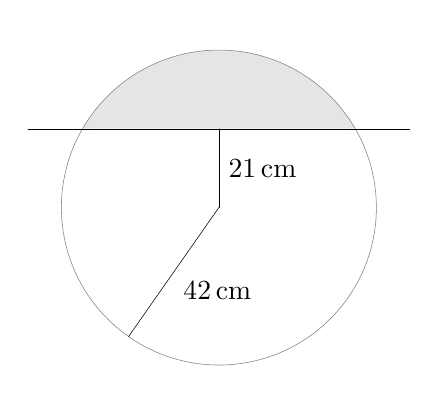
\begin{tikzpicture}[scale=0.5]
		\tkzDefPoint(0,0){A}
		\tkzDefPoint(0,4){B}
		\tkzDefPointBy[rotation=center A angle 60](B)
		\tkzGetPoint{C}
		\tkzDefPointBy[rotation=center A angle -60](B)
		\tkzGetPoint{D}
		\tkzFillSector[fill=gray!20](A,D)(C)
		\tkzDrawCircle(A,B)
		\tkzDrawPolygon[white,fill=white](A,C,D)
		\tkzDrawLine(C,D)
		\tkzDefMidPoint(C,D)
		\tkzGetPoint{E}
		\tkzDrawSegment(A,E)
		\tkzLabelSegment[right](A,E){$\SI{21}{cm}$}
		\tkzDefPointBy[rotation=center A angle 145](B)
		\tkzGetPoint{F}
		\tkzDrawSegment(A,F)
		\tkzLabelSegment[below right](A,F){\SI{42}{cm}}
	\end{tikzpicture}
	\vspace{-20pt}
\end{wrapfigure}
Farmer John made a mooshroom pizza for the cows.
(Mooshroom pizzas are ethically sourced and don't contain mooshroom meat.
They're called mooshroom pizzas because they contain mushrooms farmed from mooshrooms.)
Bessie tried to slice it, but she failed miserably, resulting in the cut shown in the following figure.
If the radius of the pizza is $\SI{42}{cm}$ and the cut is $\SI{21}{cm}$ away from the center of the pizza, what is the area of the smaller piece of pizza that was cut off?
Express your answer in exact form.

\section*{Cowcycles}
Bessie the Cow is participating in a bike race!
There are $5$ cows in the race, and they all bike at a constant speed on a circular track starting from the same position.
Bella takes $5$ minutes to complete one lap, Bessie takes $9$ minutes to complete one lap, Betty takes $3.5$ minutes to complete one lap, Betsie takes $9.8$ minutes to complete one lap, and Bossy takes $4.7$ minutes to complete one lap.
The cows have a weird tradition where once cow passes another after the race starts, they will instantaneously elbow bump each other.
In other words, each of the ${5 \choose 2} = 10$ possible pairs of cows will elbow bump each other any time they are in the exact same position after the start of the race.
For example, Bella and Bessie will elbow bump each other for the first time exactly $11.25$ minutes after the start of the race.
The cows race for $4$ hours.
How many elbow bumps will  occur in total?
Include any elbow bumps that occur exactly $4$ hours after the start of the race.

\section*{Cowtapult}
\begin{wrapfigure}{r}{0.35\linewidth}
    \vspace{-20pt}
    \centering
    \includegraphics[scale=0.25]{cowtapult.png}
    \vspace{-20pt}
\end{wrapfigure}
Cowboy Alex's barn is being attacked!!!!!
The enemy cows are in a cart that's currently $80$ meters north and $50$ meters east of the barn, and it is traveling west at $10$ meters per second.
Bessie the Cow is operating a cowtapult that is $15$ meters north of the barn.
The cowtapult launches a hay bale with a horizontal speed of $20$ meters per second in a direction that is $30$ degrees west from north.
Bessie wants to hit the enemy cart using the cowtapult.
When should she launch the hay bale?
Express your answer as a decimal in seconds, rounded to three digits after the decimal point.

\section*{Cowputing}
Bessie the Cow's new computing class has $N$ students.
If she kicks out $3$ students, she can split the students into groups of $8$.
If she adds $11$ students (to the original class of $N$ students), she can evenly split the students into groups of $5$.
If she adds $5$ students (to the original $N$ students), she can split the students into groups of $17$.
If she adds $1$ student, she can divide the students into $4$ groups each containing the same number of students.
What is the \textbf{second} smallest possible value of $N$?

\section*{Moodern Art}
\begin{wrapfigure}{r}{0.35\linewidth}
	\vspace{-20pt}
	\centering
	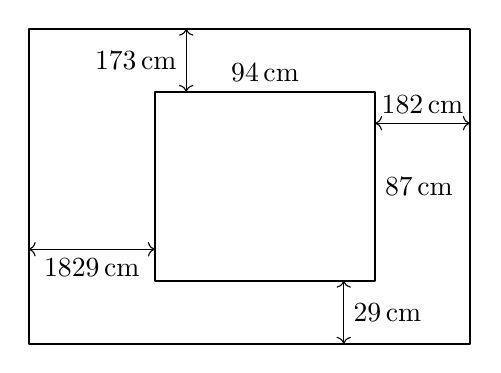
\begin{tikzpicture}[scale=0.8]
		\tkzDefPoint(0,0){A}
		\tkzDefPoint(0,5){B}
		\tkzDefPoint(7,5){C}
		\tkzDefPoint(7,0){D}
		\tkzDrawPolygon[thick](A,B,C,D)

		\tkzDefPoint(2,1){E}
		\tkzDefPoint(2,4){F}
		\tkzDefPoint(5.5,4){G}
		\tkzDefPoint(5.5,1){H}
		\tkzDrawPolygon[thick](E,F,G,H)
		\tkzLabelSegment[above](F,G){$\SI{94}{cm}$}
		\tkzLabelSegment[right](G,H){$\SI{87}{cm}$}

		\tkzDefPoint(0,1){I}
		\tkzDefPoint(2,5){J}
		\tkzDefPoint(7,4){K}
		\tkzDefPoint(5.5,0){L}
		\tkzDrawSegment[thin,arrows=<->]([yshift=0.5cm]E,[yshift=0.5cm]I)
		\tkzLabelSegment[below]([yshift=0.5cm]E,[yshift=0.5cm]I){$\SI{1829}{cm}$}
		\tkzDrawSegment[thin,arrows=<->]([xshift=0.5cm]F,[xshift=0.5cm]J)
		\tkzLabelSegment[left]([xshift=0.5cm]F,[xshift=0.5cm]J){$\SI{173}{cm}$}
		\tkzDrawSegment[thin,arrows=<->]([yshift=-0.5cm]G,[yshift=-0.5cm]K)
		\tkzLabelSegment[above]([yshift=-0.5cm]G,[yshift=-0.5cm]K){$\SI{182}{cm}$}
		\tkzDrawSegment[thin,arrows=<->]([xshift=-0.5cm]H,[xshift=-0.5cm]L)
		\tkzLabelSegment[right]([xshift=-0.5cm]H,[xshift=-0.5cm]L){$\SI{29}{cm}$}
	\end{tikzpicture}
	\vspace{-20pt}
\end{wrapfigure}
Bessie the Cow created a new painting.
It is in the shape of a rectangle $87$ centimeters tall and $94$ centimeters wide.
She hangs it on a rectangular wall such that the top edge of the painting is $173$ centimeters away from the top edge of the wall, the left edge of the painting is $1829$ centimeters away from the left edge of the wall, the right edge of the painting is $182$ centimeters away from the right edge of the wall, and the bottom edge of the painting is $29$ centimeters away from the bottom edge of the wall.
What is the area of the part of the wall that is not covered by the painting?

\section*{woC}
Bessie the Cow chooses an integer randomly and uniformly from $1000$ to $8375$ inclusive, reverses the digits, then discards any leading zeros.
What is the expected value of the result?
Express your answer in exact form.

\section*{Cowloring}
\begin{wrapfigure}{r}{0.35\linewidth}
    \vspace{-20pt}
    \centering
    \includegraphics[scale=0.35]{cowloring.png}
    \vspace{-20pt}
\end{wrapfigure}
Bessie the Cow found apiece of paper with this figure printed on it and she wants to color it using red, green, and/or blue.
In how many ways can she doe this if the orientation of the figure doesn't matter?
Each region in the figure must have exactly one of the three colors.
Two colorings are considered equivalent if one can be obtained by rotating the other.

\section*{Cownt the Calfs}
``I see you've got a new calf,'' said Cowboy Alex, peering probingly into Farmer Julia's cow farm.
``Its tail is white too, like my socks.
How many calves do you have?'' \\[0.25cm]
``Not a lot,'' said Farmer Julia.
``Rancher Emily next door has twenty, which is more than what I've got.'' \\[0.25cm]
``You still haven't told me how many calves you have!'' Cowboy Alex exclaimed. \\[0.25cm]
Farmer Julia, who knew that Cowboy Alex was something of an amateur mathematician, said, ``Well \ldots let me put it like this.
If you choose two distinct calves of mine at random, the probability that both of them have white tails is exactly one-half.'' \\[0.25cm]
How may calves does Farmer Julia have in total?

\section*{Cowld}
\begin{wrapfigure}{r}{0.35\linewidth}
    \vspace{-20pt}
    \centering
	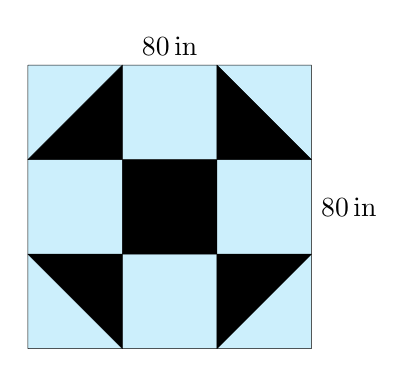
\begin{tikzpicture}[scale=0.4]
		\tkzDefPoint(0,0){A}
		\tkzDefPoint(9,0){B}
		\tkzDefSquare(A,B)
		\tkzGetPoints{C}{D}
		\tkzDrawPolygon[fill=cyan!20](A,B,C,D)
		\tkzLabelSegment[above](C,D){$\SI{80}{in}$}
		\tkzLabelSegment[right](B,C){$\SI{80}{in}$}

		\tkzDefPoint(3,3){E}
		\tkzDefPoint(6,3){F}
		\tkzDefSquare(E,F)
		\tkzGetPoints{G}{H}
		\tkzDrawPolygon[fill=black](E,F,G,H)
		
		\tkzDefPoint(3,0){I}
		\tkzDefPoint(6,0){J}
		\tkzDefPoint(9,3){K}
		\tkzDefPoint(9,6){L}
		\tkzDefPoint(6,9){M}
		\tkzDefPoint(3,9){N}
		\tkzDefPoint(0,6){O}
		\tkzDefPoint(0,3){P}
		\tkzDrawPolygon[fill=black](E,I,P)
		\tkzDrawPolygon[fill=black](F,J,K)
		\tkzDrawPolygon[fill=black](G,L,M)
		\tkzDrawPolygon[fill=black](H,N,O)
	\end{tikzpicture}
	\vspace{-20pt}
\end{wrapfigure}
Cowboy Alex wants to make a blanket for his cows with a specific pattern because they are cold.
If the blanket uses the pattern $36$ times and one side of the pattern is $80$ inches, at least how many inches of black fabric will he need to make blankets for $20$ cows?

\section*{The Great Cow Chase of 2021}
Oh no!
Kiran the cow is making an escape!
Kiran is running at $\SI{20}{mph}$.
Kiran is currently $10$ miles from the end of the fence so Rancher Cedric knows Kiran will make a turn.
The left side of the fence is $30$ miles long.
To catch up with Kiran faster, he decides to ride his horse diagonally across the field.
He is riding his horse at $\SI{30}{mph}$ to catch Kiran.
How long will it take for him to catch the cow?

\section*{Cowyon}
\begin{wrapfigure}{r}{0.35\linewidth}
	\vspace{-20pt}
	\centering
	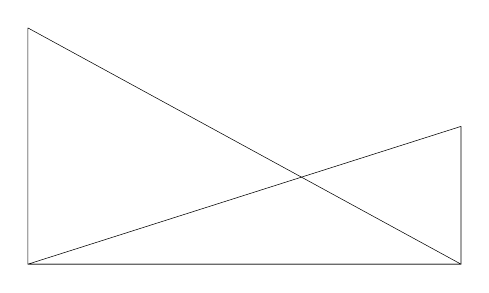
\begin{tikzpicture}[scale=0.25]
		\tkzDefPoint(0,0){A}
		\tkzDefPoint(0,12){B}
		\tkzDefPoint(22,0){C}
		\tkzDefPoint(22,7){D}
		\tkzDrawPolygon(A,B,C)
		\tkzDrawPolygon(A,C,D)
	\vspace{-20pt}
	\end{tikzpicture}
\end{wrapfigure}
A widely-known bazaar is situated in a great canyon, with vertical cliffs on both sides.
One cliff is $700$ meters high, while the other is $1200$ meters high.
A zip line runs from the foot of each cliff to the top fo the other cliff; the zip lines are perfectly straight.
At what height above the ground do the two cables meet?

\section*{Rowdy Cow}
After Rancher Cedric caught Kiran the cow in the Great Cow Chase, Kiran decided to trample the grass and terrorize the chickens.
Rancher Cedric had enough, and he decided to lock him in a pen.
The pen is in the shape of an equilateral triangle, and each side is $500$ meters long.
The rowdy cow is tied to one corner, so that the portion of the field it can reach is exactly half of the total area.
Assume that Kiran and the rope have zero width.
How long is the rope?

\section*{The Farmer's Cownundrum}
\begin{wrapfigure}{r}{0.35\linewidth}
	\vspace{-20pt}
	\centering
	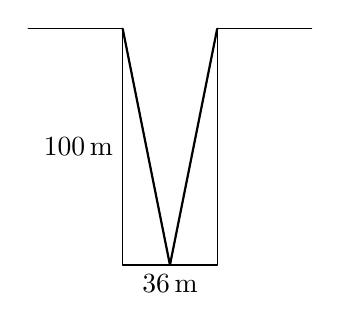
\begin{tikzpicture}[scale=0.3]
		\tkzDefPoint(0,10){A}
		\tkzDefPoint(4,10){B}
		\tkzDefPoint(4,0){C}
		\tkzDefPoint(8,0){D}
		\tkzDefMidPoint(C,D)
		\tkzGetPoint{E}
		\tkzDefPoint(8,10){F}
		\tkzDefPoint(12,10){G}

		\tkzDrawSegments[thin](A,B B,C C,D D,F F,G)
		\tkzDrawSegments[thick](B,E E,F)
		\tkzLabelSegment[left](B,C){$\SI{100}{m}$}
		\tkzLabelSegment[below](C,D){$\SI{36}{m}$}
	\end{tikzpicture}
	\vspace{-20pt}
\end{wrapfigure}
Farmer Robert submits the blueprints for his cow farm to his contractor, but the contractor misreads the information!
The Farm is now separated by a $36$ meter long divide that is $100$ meters deep.
Robert has a huge ego, so he believes that the bridge should be shaped in a V because it is the first letter of his last name.
Assuming that each side of the V is equal in length and reaches the floor, how long would the bridge be in meters?

\section*{Moocraft}
Bessie the Cow's new hobby is trying to beat the video game Moocraft as fast as possible.
On the first day, Bessie finished Moocraft in $40$ minutes.
The next day, Bessie finished Moocraft in three-fourths of the time it took the day before.
On the third day, Bessie's time is five-sevenths of the time on the second day.
How many seconds did it take for Bessie to complete Moocraft on the third day?
Round your answer to the nearest integer.

\section*{Moss-cow}
Bessie the Cow is currently staying in London during a world tour to find the tastiest grass.
She prepares to visit Moscow, but wants to know how long it will take to get there.
The route from London to Moscow is $1600$ miles long.
First, Bessie will ride a train moving at $60$ miles per hour.
If the whole journey took $19.5$ hours, how long did Bessie spend on the plane?
Assume that the time it takes for Bessie to transfer from the plane to the train is negligible.

\section*{Revomootion}
Farmer John's cows are planning revolution to overthrow him!
The $42$ cows plan to distribute themselves among $6$ pastures.
To make sure Farmer John doesn't get suspicious, there must be at least two cows in each pasture, each pasture must have a different number of cows, and pasture can have exactly $3$ or $3$ cows.
To help the cows calculate their chance of succeeding, find the greatest number of cows that can be in any one pasture.

\section*{Bessie Buys Brass Bells by the Big Barn}
Bessie the Cow is interested in buying new bells for herself and her friends.
The Barnyard Bazaar sells three different types of bells: blue bells, brown bells, and burgundy bells.
Each type of bell has a constant cost per bell.
Three blue bells and one brown bell would cost a total of $35$ cents.
Two brown bells and four burgundy bells would cost a total of $28$ cents.
One blue bell and two burgundy bells would cost a total of $9$ cents.
How much would four blue bells and three brown bells cost?

\section*{Moorio Kart}
Cowboy Alex gave Bessie the Cow a new racing game called Moorio Kart!
She let all one hundred of her cow friends play, and then asked each cow whether they liked each of the three courses.
$65$ cows said they liked Bowser's Cowstle, $75$ cows said they liked Cowconut Mall, and $85$ cows said they liked Moo Moo Meadows.
What is the fewest number of cows that could have said they liked all three courses?

\section*{Cownt the Rectangles}
\begin{wrapfigure}{r}{0.35\linewidth}
	\vspace{-20pt}
	\centering
	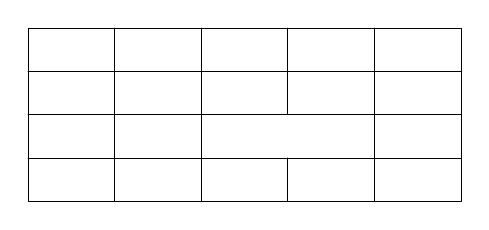
\begin{tikzpicture}[scale=0.55]
		\tkzDefPoint(0,0){A}
		\tkzDefPoint(0,4){B}
		\tkzDefPoint(10,4){C}
		\tkzDefPoint(10,0){D}
		\tkzDrawPolygon(A,B,C,D)

		\tkzDefPoint(0,1){E}
		\tkzDrawSegment(E,[xshift=10cm]E)
		\tkzDefPoint(0,2){F}
		\tkzDrawSegment(F,[xshift=10cm]F)
		\tkzDefPoint(0,3){G}
		\tkzDrawSegment(G,[xshift=10cm]G)

		\tkzDefPoint(2,0){H}
		\tkzDrawSegment(H,[yshift=4cm]H)
		\tkzDefPoint(4,0){I}
		\tkzDrawSegment(I,[yshift=4cm]I)
		\tkzDefPoint(6,0){J}
		\tkzDrawSegment(J,[yshift=1cm]J)
		\tkzDrawSegment([yshift=2cm]J,[yshift=4cm]J)
		\tkzDefPoint(8,0){K}
		\tkzDrawSegment(K,[yshift=4cm]K)
	\end{tikzpicture}
	\vspace{-20pt}
\end{wrapfigure}
Bessie the Cow found a piece of paper with the following figure printed on it.
She wants to know how many rectangles are in the figure.
Help her by finding the number of rectangles of any size that is in this figure, including rectangles which contain multiple smaller rectangles.

\section*{Cowlifornia}
Bessie the Cow and her siblings have always dreamed of living in Cowlifornia.
However, Bessie has a lot of siblings, so it'll be hard to find a farm they van all moove to!
Bessie has two more sisters than brothers.
Her brother, Kiran, has twice as many sisters as brothers.
How many siblings does Bessie have?

\section*{Moogic}
\begin{wrapfigure}{r}{0.35\linewidth}
	\vspace{-20pt}
	\centering
	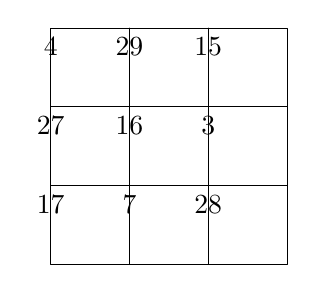
\begin{tikzpicture}
		\tkzDefPoint(0,0){A}
		\tkzDefPoint(3,0){B}
		\tkzDefSquare(A,B)
		\tkzGetPoints{C}{D}
		\tkzDrawPolygon(A,B,C,D)

		\tkzDefPoint(1,3){E}
		\tkzDefPoint(2,3){F}
		\tkzDrawSegment(E,[yshift=-3cm]E)
		\tkzDrawSegment(F,[yshift=-3cm]F)

		\tkzDefPoint(0,2){G}
		\tkzDefPoint(0,1){H}
		\tkzDrawSegment(G,[xshift=3cm]G)
		\tkzDrawSegment(H,[xshift=3cm]H)

		\tkzDefPoint(1,2){J}
		\tkzDefPoint(2,2){K}
		\tkzDefPoint(1,1){L}
		\tkzDefPoint(2,1){M}

		\foreach \name\value in {D/$4$, E/$29$, F/$15$, G/$27$, J/$16$, K/$3$, H/$17$, L/$7$, M/$28$}
		{
			\tkzLabelPoint(\name){\value}
		}


	\end{tikzpicture}
	\vspace{-20pt}
\end{wrapfigure}
Bessie the Cow wanted to learn how to do magic, but she got distracted on the internet and ended up learning about magic squares.
In a magic square, the sum of the numbers in each row, each column, and the two main diagonals are the same.
If exactly two numbers are changed in this grid, the result is a magic square.
Which two numbers must be changed and what values should they be changed?
\end{document}
